\section{Ambiente de contratação Regulado e Ambiente de Contratação Livre}

\subsection{introdução}

Conforme já mencionado em outros pontos deste livro, o mercado elétrico brasileiro é inteiramente baseado em contratos, e estes podem ser feitos no \textbf{ambiente de contratação regulado} (ACR) ou no \textbf{ambiente de contratação livre} (ACL). O ponto de encontro entre estes dois mercados está na CCEE, que faz o balanço semanal de todos os contratos. Este capítulo tem como objetivo apresentar uma discussão sobre estes dois mercados. 

O sistema elétrico é baseado em contratos porque não uma vez que um elétron é despachado de um gerador, não temos como controlar para onde ele vai, ou seja, uma vez no sistema, tudo se torna uma coisa só. Porém, podemos medir as pontas do sistema, ou seja, sabemos quando foi gerado e quanto foi consumido por cada agente do sistema. Assim, suponha que um gerador $G$ tenha um contrato de 100MW com um consumidor $C$. Esta informação estará na CCEE, se o gerador $A$ gerar algo diferente de 100MW, esta diferença será liquidada pelo \textbf{preço de liquidação de diferenças} (PLD), também conhecido como preço spot. O mesmo vale para o consumidor. Assim, é possível ter um controle sobre a oferta e a demanda do sistema e um melhor planejamento para sua expansão. 

Antes de irmos para o ACR, vamos discutir algumas características do sistema brasileiro que vão tornar a compreensão do todo mais fácil. Já sabemos que o Brasil possui um sistema elétrico hidrotérmico, com uma participação maior de hidrelétricas\footnote{Este cenário está mudando aos poucos com a introdução de novas térmicas e de fontes renováveis.}, portanto, faz todo o sentido que o preço da energia esteja ligado aos fatores determinantes da geração hídrica. Nosso preço spot (PLD) é calculado semanalmente através de modelos de otimização como aqueles vistos nos capítulos anteriores. Porque semanal? Porque o preço não pode ser definido pelo valor da ultima transação, como acontece em bolsas  de valores? A resposta está nas próprias características do setor. Entende-se que a eficiência e a capacidade de fornecimento de nosso sistema está altamente ligado ao volume dos reservatórios de nossas hidrelétricas. Reservatórios demoram tanto para encher quanto para esvaziar, ou seja, o estado do sistema não muda muito dentro de poucos dias, ou até poucas semanas. Por este motivo, não faz muito sentido introduzir preços horários ou diários como em outros países, isso geraria uma volatilidade prejudicial ao sistema. Falando em volatilidade, podemos concluir com o que foi dito, que PLD, apesar de mudar pouco em dias ou semanas, pode ter uma volatilidade muito elevada quando olhamos para meses ou anos. A figura \ref{fig:aula12_2} mostra, em vermelho o volume dos reservatórios e em azul o PLD. Podemos ver que em momentos em que o sistema está estressado, como no racionamento de 2001, o PLD é muito alto e muito volátil, e o volume dos reservatórios tende a estar abaixo do esperado para aquela época do ano. Devemos abrir um parênteses aqui para fazer uma observação: o sistema com um preço como o nosso possui longos períodos de PLD muito próximo a zero, portanto, o PLD não é um bom sinalizador para a necessidade de expansão do sistema.   


\begin{figure}[H]
\begin{centering}
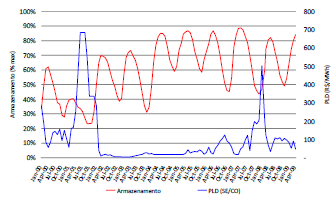
\includegraphics[scale=1.0]{aula12_2}\protect\caption{\label{fig:aula12_2} PLD X Volume dos Reservatórios}
\end{centering}
\end{figure}

O consumo de energia está altamente ligado à atividade econômica do país, portanto deve-se considerar o crescimento esperado no planejamento da expansão do sistema. No caso de países emergentes, como é o caso do Brasil, isso não é uma tarefa fácil. As taxas de crescimento por aqui tendem a ser maiores do que aquelas em países desenvolvidos. Isso faz com que em um prazo de aproximadamente 20 anos, nosso consumo de energia dobre, ou seja, temos que dobrar o tamanho de nosso sistema. Da para ter uma ideia do quanto isso é difícil? São bilhões de dólares em investimentos e planejamento. Usinas muitas vezes são demoradas para construir, portanto o planejamento deve ser feito com antecedência e precisão. A oferta deve correr atrás da demanda, que cresce muito rápido. A figura \ref{fig:aula12_3} ilustra o que foi dito. Ela mostra a demanda anual de energia no Brasil. Podemos ver que de 1992 até 2012 a demanda dobrou. Para dificultar ainda mais, as taxas de crescimento do Brasil variam muito. Entre 2007 e 2015, tivemos taxas de $-2\%$ a $8\%$. Portanto, um mau planejamento pode levar a um excesso de oferta de energia.  


\begin{figure}[H]
\begin{centering}
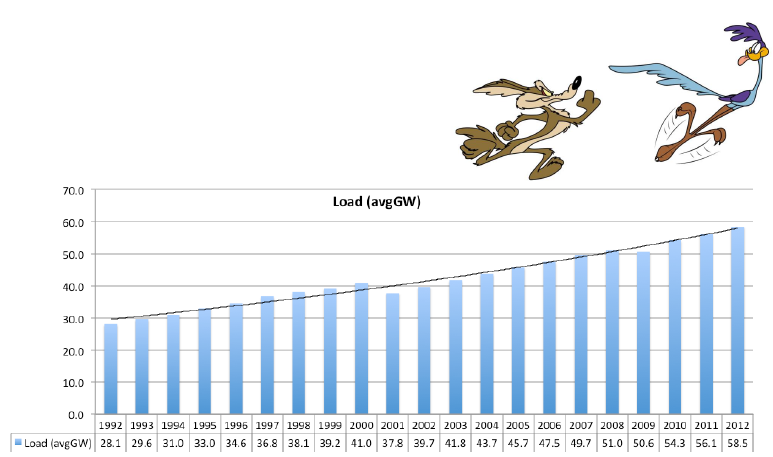
\includegraphics[scale=0.6]{aula12_3}\protect\caption{\label{fig:aula12_3} Demanda anual de energia no Brasil}
\end{centering}
\end{figure}

\subsection{Ambiente Regulatório}

O sistema elétrico brasileiro foi construído no contexto descrito acima. Nos temos um sistema com pouca capacidade de resposta à variações de curto prazo na demanda, e a regulação do sistema levou isso em conta. É aí que entram os contratos de energia. Eles surgem com o objetivo de reduzir o risco do sistema e de seus agentes. Por exemplo, uma vez que uma usina possui um contrato, ela tem uma garantia de receita, e fica mais fácil conseguir um financiamento mais barato. 

Para garantir a capacidade de suprimento, todo o sistema brasileiro deve estar lastreado. Ou seja, toda demanda deve ter um certificado de $100\%$ de sua energia. Para tornar isso possível criou-se o conceito da \textbf{garantia física}, ou seja, quando um determinado gerador agrega de fato ao sistema. A garantia física é um teto para o quanto cada gerador pode vender em contratos, que é menos do que $100\%$. de sua capacidade. Imagine uma hidrelétrica, ela está sujeita ao regime climático do Brasil, portanto, nos períodos secos ela agrega menos ao sistema do que em períodos de chuva. Sendo assim, ela não pode contratar sua capacidade máxima, que geralmente só pode ser garantida em períodos chuvosos. No caso de térmicas, se elas fazem parte da base, ou seja, tem um curto marginal barato e estão sempre ligadas, suas garantias físicas são muito próximas à $100\%$. Entretanto, térmicas caras que são ligadas raramente possuem uma garantia física menor. 
Além disso, ao montar um sistema baseado em lastro os contratos de longo prazo se tornam um garantidor financeiro, os investimento se tornam mais atrativos. 

\subsection{O ACR e os Leilões}

Tudo que foi dito até agora vale tanto para o ACR quanto para o ACL. Agora vamos focar nas características apenas do primeiro. No ACR a energia é comprada dos geradores por distribuidoras em leilões, ou seja, não há contato direto entre consumidor e gerador. Nós, consumidores, compramos nossa energia das distribuidoras e pagamos uma tarifa por nosso consumo. Nós, pequenos consumidores, somos obrigados a estar sob uma distribuidora, consumidores maiores podem escolher de onde compram sua energia. 

As distribuidoras de energia devem comprar seus contratos de energia em leilões. Elas declaram sua demanda, e o leilão é realizado de forma a obter o menor preço possível pelo MHw. Os geradores expressam seus preços em várias etapas para assegurar que não haja assimetria de informação e que os preços verdadeiros sejam os preços finais dos leilões. A figura \ref{fig:aula12_4} mostra a configuração atual dos leilões de energia no Brasil. Os leilões podem ser classificados em dois grandes grupos: 1) leilões de energia existente, onde participam geradores que já foram construídos, em geral para renovação de contratos vencidos; 2) leilões de energia nova, neste tipo de leilão potenciais geradores buscam contratos para tornar viável a construção de suas usinas. Os leilões A-3 e A-5 são leilões feitos hoje para contratos que entrarão em vigor daqui a 3 ou 5 anos, de forma que os vencedores dos leilões de energia nova tenham tempo para buscar financiamento e construir suas usinas. Lembrando que apenas a garantia física pode ser vendida nos leilões afim de assegurar o lastro do sistema.  

\begin{figure}[H]
\begin{centering}
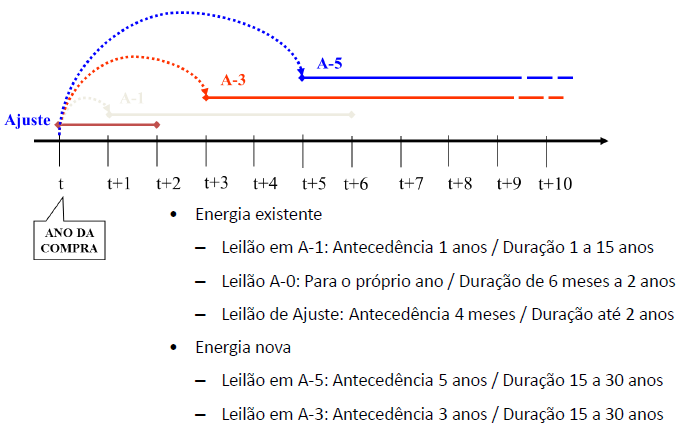
\includegraphics[scale=0.6]{aula12_4}\protect\caption{\label{fig:aula12_4} Configuração dos leilões no Brasil}
\end{centering}
\end{figure}

O ambiente regulado corresponde a $70\%$ do mercado brasileiro de energia. O ambiente livre possui uma parcela maior e características diferentes, onde agentes podem negociar livremente os contratos. Os leilões possuem a vantagem de atuarem como ferramenta para descobrir o preço verdadeiro da energia, algo impossível de ser feito por um planejador central. Para maiores informações sobre a teoria de leilões, estudem a teoria de desenho de mecanismos. Leilões não são nada mais do que mecanismos de incentivo que visam equilibrar oferta e demanda e revelar preços. Abaixo identificamos os tipos básicos de leilões:

\begin{itemize}
\item Leilões podem ser de compra ou de venda,
\item podem ser abertos (lances são públicos) ou fechados (lances secretos),
\item podem conter um objeto ou múltiplos objetos,
\item Podem ser iterativos, com preços ascendentes (leilão inglês) ou descendentes (leilão holandês),
\item Podem ter preço uniforme (o preço final vale para todos os vencedores) ou discretos (cada vencedor tem o preço de seu lance).
\end{itemize}

Existem várias coisas interessantes por trás da teoria dos leilões, por exemplo, a situação conhecida como maldição do vencedor. Imagine que você tem um projeto de uma termelétrica que após exaustivos estudos pode aceita no mínimo 100 reais por MHw para ser viável. O leilão está agora em 120 reais, você está tranquilo. O tempo vai passando e as pessoas vão dando os lances, e o preço chega a 102 reais. Você começa a ficar nervoso mas continua dando o seu lance. Finalmente o preço chega a 99 reais. Você deveria parar, mas no calor do momento, acaba continuando, porque um realzinho a menos da para contornar. Quando menos percebe, está fazendo lances de 85 reais, e vence o leilão. Na hora você comemora, mas logo percebe que arrumou um grande problema para sua vida, pois só consegue vender energia a 100 reais por MHw. Os desenhos de leilões devem buscar evitar esse tipo de comportamento. 

Vamos voltar agora para a figura \ref{fig:aula12_4}. Toda a ideia da expansão do sistema pode ser vista nessa figura. Os leilões A-3 tem como principal alvo termelétricas e renováveis, e o A-5 hidrelétricas que demoram mais para serem construídas. Entretanto, existem outras coisas por trás da separação dos leilões de energia nova em dois horizontes de tempo. Lembramos que a demanda futura é algo incerto, portanto seria muito arriscado deixar tudo por conta do leilão A-5. Assim o A-3 serve também como ajuste. 

Além disso, existem dois tipos de contratos oriundos dos leilões, os contratos por quantidade e os contratos por disponibilidade. Os primeiros tem como foco hidrelétricas e renováveis que são obrigadas a despachar tudo que produzem, como é o caso das eólicas. Os contratos, nesse caso, são diretamente para a quantidade de energia gerada. Já no caso dos contratos de disponibilidade, é como se estivéssemos pagando para alguém existir e estar disponível para quando for preciso. Esse é o caso de termelétricas, que devem ficar prontas para quando o ONS despacha-las. Abaixo apresentamos os requisitos básicos para participar dos leilões de energia nova.

\begin{itemize}
\item Ficha de dados: resumo dos principais dados técnicos,
\item Parecer de acesso: emitido pelo ONS, EPE ou distribuidora,
\item Licença ambiental prévia,
\item Estudos de impactos ambientais,
\item Termo de compromisso realizado com o fornecedor de combustível (para usinas que precisam de combustível),
\item Direito de uso do local onde será feito o empreendimento,
\item Memorial descritivo,
\item Certificados de medições anemométricas e estimativa de produção no caso de eólicas,
\item outros.
\end{itemize}

Além dos itens acima, existem outros mecanismos para garantir que a usina vencedora do leilão será efetivamente construída e os contratos honrados. Uma vez feito tudo isso, vamos analisar como são feitos os lances. Para colocar todos os competidores de leilão de uma forma que seja possível compara-los, foi criado o índice de custo e benefício (ICB). Dentro deste índice entram diversas informações sobre os geradores, e o ICB será o lance. A equação (\ref{eq12-1}) apresenta o ICB. O primeiro termo, $RF$, representa os custos fixos dos geradores, ele é o único valor que pode ser alterado pelo competidor, ou seja, o lance é feito em $RF$. O $COP$ diz respeito a expectativa de gastos com a operação das usinas, no caso das térmicas, com combustíveis e no caso geral, manutenção, pagamentos de funcionários, etc. O $CEC$ estima os gastos médios com liquidação na CCEE e $GF$ é a garantia física. No numerados temos custos, e no denominados benefícios. Todos os termos da equação (\ref{eq12-1}) são calculados antes do leilão por entidades regulatórias. 

\begin{equation}
\label{eq12-1}
ICB=\frac{RF+COP(g,c)+CEC(g,c)}{GF(g,c)}
\end{equation}

A figura \ref{fig:aula12_5} resume tudo que vimos até agora sobre leilões. Vamos agora tratar, de forma um pouco mais específica, como acontecem os leilões de energia nova no brasil. 

\begin{figure}[H]
\begin{centering}
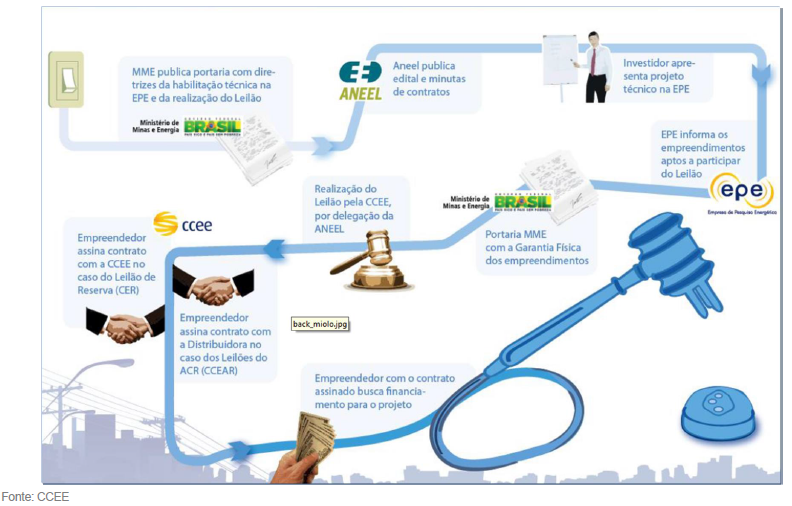
\includegraphics[scale=0.6]{aula12_5}\protect\caption{\label{fig:aula12_5} Como são organizados os leilões}
\end{centering}
\end{figure}

\subsection{Leilões de Energia Nova}

Os leilões de energia nova começam com as distribuidoras definindo perante a CCEE/ANEEL quando desejam contratar de energia. O leilão é feito baseado nesta quantidade, como mostra a figura \ref{fig:aula12_6}. A quantidade demandada por cada distribuidora e a quantidade total demandada é mantida em segredo, inclusive durante a realização do leilão. 

O leilão é então realizado em três fases. A primeira diz respeito apenas às hidrelétricas, e define seus direitos de concessão. A segunda fase é mostrada na figura \ref{fig:aula12_7}. Ela é feita para hidrelétricas e termelétricas separadamente. Tudo começa com uma demanda de referência, que é maior do que a demanda verdadeira das distribuidoras. O leilão é feito com preços decrescentes, e os lances são feitos até que a demanda de referência seja atingida. Quando isto ocorre, todos os que estão acima da demanda de referência são descartados por ordem de mérito com base no ICB. Nesta fase os preços são uniformes. 

\begin{figure}[H]
\begin{centering}
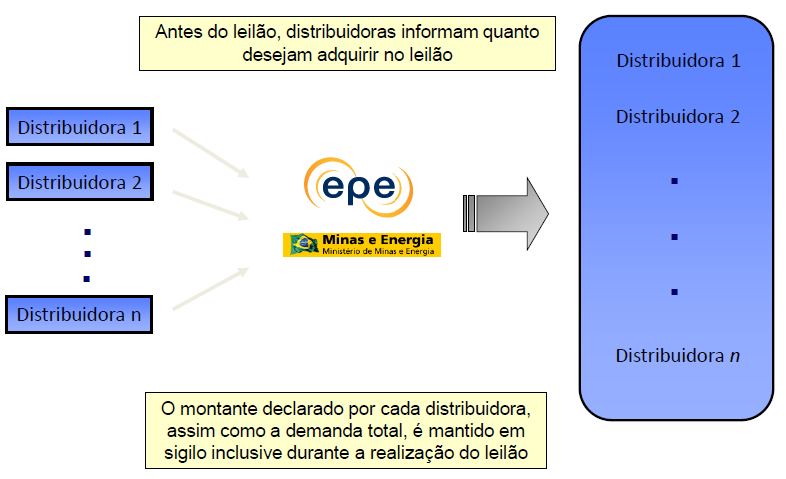
\includegraphics[scale=0.7]{aula12_6}\protect\caption{\label{fig:aula12_6} Distribuidoras antes do leilão começar}
\end{centering}
\end{figure}

\begin{figure}[H]
\begin{centering}
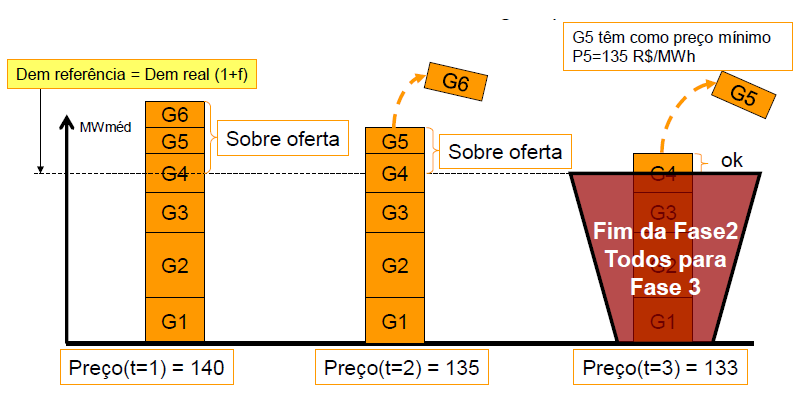
\includegraphics[scale=0.7]{aula12_7}\protect\caption{\label{fig:aula12_7} Leilões: Fase 2}
\end{centering}
\end{figure}

Os leilões tem ainda uma terceira fase, esquematizada nas figuras \ref{fig:aula12_8} e \ref{fig:aula12_9}. Nela, os competidores tem 15 minutos para oferecer preços menores do que o preço ao final da fase dois. São selecionados os empreendimentos mais baratos até que a demanda real seja atendida. Finalmente, na fase final (\ref{fig:aula12_10}) os contratos são assinados diretamente entre os geradores e as distribuidoras de acordo com a demanda e a oferta de cada agente. 

\begin{figure}[H]
\begin{centering}
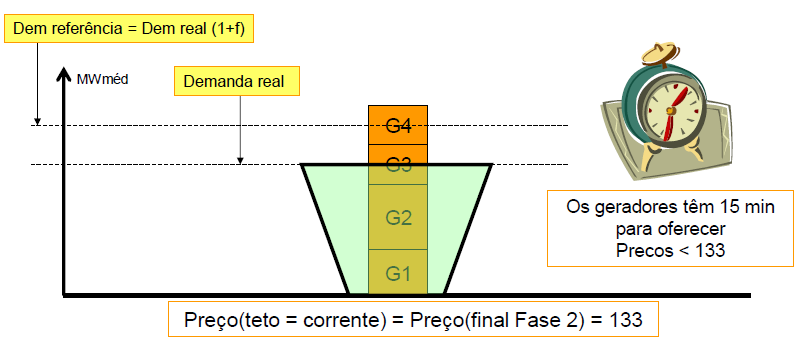
\includegraphics[scale=0.7]{aula12_8}\protect\caption{\label{fig:aula12_8} Leilões: Fase 3 - parte 1}
\end{centering}
\end{figure}

\begin{figure}[H]
\begin{centering}
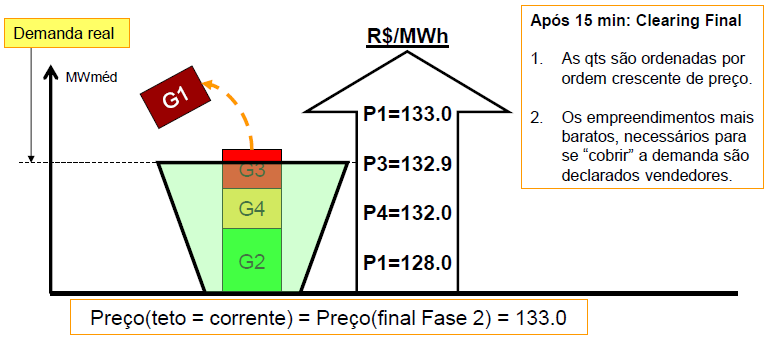
\includegraphics[scale=0.7]{aula12_9}\protect\caption{\label{fig:aula12_9} Leilões: Fase 3 - parte 2}
\end{centering}
\end{figure}


\begin{figure}[H]
\begin{centering}
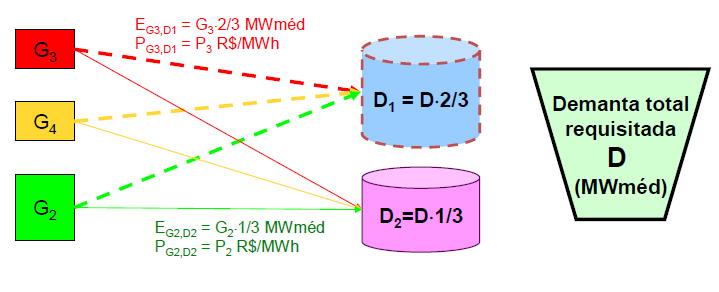
\includegraphics[scale=0.7]{aula12_10}\protect\caption{\label{fig:aula12_10} Leilões: Fechamento}
\end{centering}
\end{figure}

Existem outros casos especiais de leilões, por exemplo os de energia de reserva, que vem sido utilizados para incentivar fontes renováveis e garantir uma energia suplementar para o sistema. Além disso, a energia de reserva não forma lastro contratual. Exceto pelas características citadas acima, todo o resto é igual aos leilões já mencionados. 

\subsection{Leilões de Energia Existente e Projetos Específicos}

Os leilões de energia existente tem como objetivo recontratar energia que já instalada. Estes leilões são de curto e médio prazo, e visam atender a demanda atual. Os leilões A-1 são realizados anualmente e os contratos passam a valer no início do ano seguinte, e os leilões de reserva são realizados no decorrer do ano com início imediato de suprimento. No caso dos A-1, os contratos podem ter duração de 1 até 15 anos, já os leilões de ajuste limitam os contratos a dois anos e só podem ocorrer na quantidade de $1\%$ ou menos da demanda. 

Os contratos de energia existente geram uma flexibilidade nova para as distribuidoras, pois podem ser cancelados se algum consumidor deixar a distribuidora para ir para o ACL, e além disso pode ser reduzido em $4\%$ ao ano para compensar a incerteza na demanda. Porém, estes mecanismos geram um risco a mais para o gerador existente, pois este pode perder seu contrato. 

O Brasil possui muita experiência com leilões de energia nova. Já aconteceram cerca de 25 leilões deste tipo, sendo que 8 eram exclusivamente de renováveis. Entre 2008 e 2016 temos mais de 60.000Mw contratados. 

Por último, existe outro tipo de leilão que envolve projetos específicos. Este é o caso de mega-usinas hidrelétricas que envolvem um alto risco ambiental e político. Em geral, este tipo de projeto é feito pelo governo em conjunto com a sociedade, e então é licitado por meio de um leilão para que alguém possa construir e operar a nova hidrelétrica. 

Para encerrar no ACR, mostramos que a ferramenta dos leilões é a alma do ambiente de contratação regulado. Eles são capazes de assegurar o suprimento, promover transparência e aumentar a competição. Outros países estão começando a utilizar leilões em seus mercados, como é o caso do Chile, Peru, Panamá e outros. O Brasil é líder mundial em leilões de energia, com mais de 50 leilões realizados. Esta experiência está documentada pelo Banco Mundial. Entretanto, o diabo vive nos detalhes. 


\subsection{Ambiente de Contratação Livre}

No capítulo passado falamos sobre o ambiente de contratação regulado (ACR), onde as distribuidoras compram energia por meio de leilões, e vendem esta energia para os consumidores. Todo o ACR está sustentado nos leilões. Agora falaremos do ambiente de contratação livre (ACL), onde contratos podem ser negociados livremente entre gerador, comercializador e consumidor. 

O ACL oferece uma maior flexibilidade na negociação de contrato, produtos diferenciados e a possibilidade de gerência de risco. Entretanto, é um mercado onde existe uma maior assimetria de informação e regras muito complexa, principalmente quando se trata do rateio dos custos de transação. Não é qualquer consumidor que pode entrar no ACL, algumas condições devem ser atendidas. Consumidores normais só podem entrar se tiverem uma demanda superior a 3kW. Entretanto, para gerar um incentivo às fontes renováveis, foi permitido que consumidores com demanda superior a 500kW participassem do ACL desde que contratados com renováveis. Além disso, fontes renováveis tem um desconto de $50\%$ na transmissão, permitindo que a energia seja vendida a um preço menor. Em outros países as regras são diferentes, por exemplo, na Europa e na Nova Zelândia todos os consumidores podem escolher de onde compram energia. 

\subsubsection{O Mercado}

Com a criação do ACL surgiu um novo tipo de agente no mercado, o comercializador. Ele contrata energia de geradores e vende a outros geradores e a consumidores. Sua principal função é reduzir o custo de transação fazendo o casamento entre geradores e consumidores. Além disso, eles oferecem mais liquidez ao mercado e representam seus clientes junto a CCEE. A grande experiência dos comercializadores permite que eles ofereçam produtos diferenciados, como portfólios de renováveis menos ariscados do que a geração de usinas individuais. 

Um consumidor que está no ambiente regulado pode, a qualquer momento, ir para o ambiente livre. No caso contrário, ou seja, um consumidor livre deseja ir para o regulado, a distribuidora é obrigada a aceita-lo. Entretanto, ela pode pedir um tempo de até 5 anos para entrar no leilão e comprar a energia para este novo consumidor. 

Tipicamente, um contrato no ACL tem contém as seguintes informações:

\begin{itemize}
\item Volume contratado e preço,
\item Período de indexação,
\item Submercado de entrega,
\item Responsabilidade pelo risco de mercado,
\item Modulação,
\item Flexibilidades mensais,
\item Sazonalização,
\item Registro na CCEE,
\item Tavas: tetos e pisos,
\item Pagamentos, multas, etc.
\end{itemize}

O ACL ainda não possui uma bolsa de energia, portanto as negociações são feita em balcões. Isso leva a um mercado desorganizado e com muita assimetria de informação. Além disso, não existe uma entidade que ofereça as garantias financeiras asseguradas por uma bolsa de valores. Entretanto, existem alguns esboços de bolsas no Brasil, porém sem grande volume até o momento. 

Como o ACL funciona como um mercado, o preço se da pelo equilibro entre oferta e demanda, obviamente influenciado por alguns fatores externos, como o PLD. Ainda assim, o preço depende da disposição a vender do gerador e da disposição a comprar do consumidor. 

Como dito anteriormente, existe também um ACL incentivado, onde consumidores menores podem participar desde que contratados de renováveis de geração máxima de 30mW. Além disso existe um desconto de $50\%$ na transmissão para estes casos, desconto este que pode chegar até a $100\%$. A figura \ref{fig:aula13_1} mostra como essa vantagem na transmissão pode ser aproveitada. 


\begin{figure}[H]
\begin{centering}
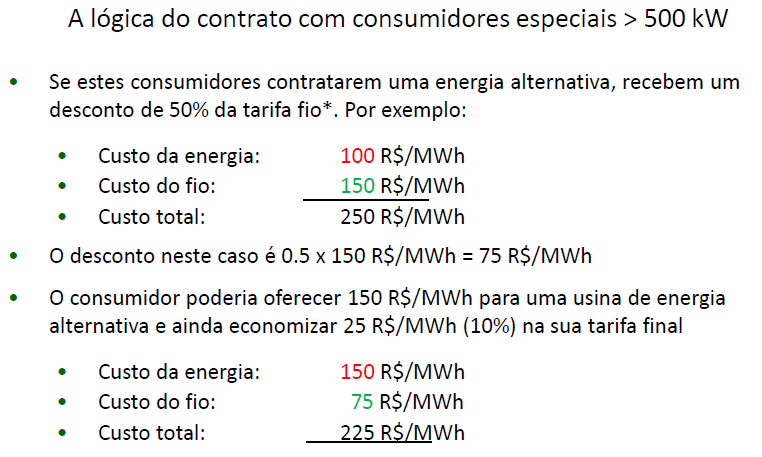
\includegraphics[scale=0.6]{aula13_1}\protect\caption{\label{fig:aula13_1} Vantagens na Transmissão de Renováveis}
\end{centering}
\end{figure}

Cada vez mais os produtos oferecidos pelo ambiente livre estão ficando mais sofisticados. Existem vários tipos de contratos e portfólios oferecidos que visam reduzir o riscos, escapar de efeitos sazonais, e outros. Por exemplo, podemos diversificar entre PCH, biomassa e eólica e ter um fluxo de energia seguro. Imagine uma PCH no sudeste, uma usina de biomassas, também no sudeste e uma eólica no nordeste. Fazendo um portfólio com esses três geradores eliminamos boa parte do risco sazonal, uma vez que suas sazonalidades são complementares. Apesar de tudo isso, observe que no ACL você está sujeito à liquidação de diferenças na CCEE, ou seja, deve contratar uma quantidade de energia, que se ultrapassada será liquidada a PLD. Este tipo de risco não existe quando estamos sob uma distribuidora.  




